\secnumbersection{CONCLUDING REMARKS} \label{sec:concluding_remarks}
The problem faced in this work is multifaceted: it requires to understand the physics behind how particle accelerators and detectors work, then analyze the algorithms to implement these physics in a computer, and finally to code these algorithms in the implementation's environment.
These different facets can also be seen in the contributions of this work.
The team of physicists at JLab see the benefit of a quicker software which allows to analyze the data produced by the detector faster, while the general community benefits from ideas related to particle accelerators, Kalman filters and state estimators in general.

    \begin{figure}[ht]
        \centering
        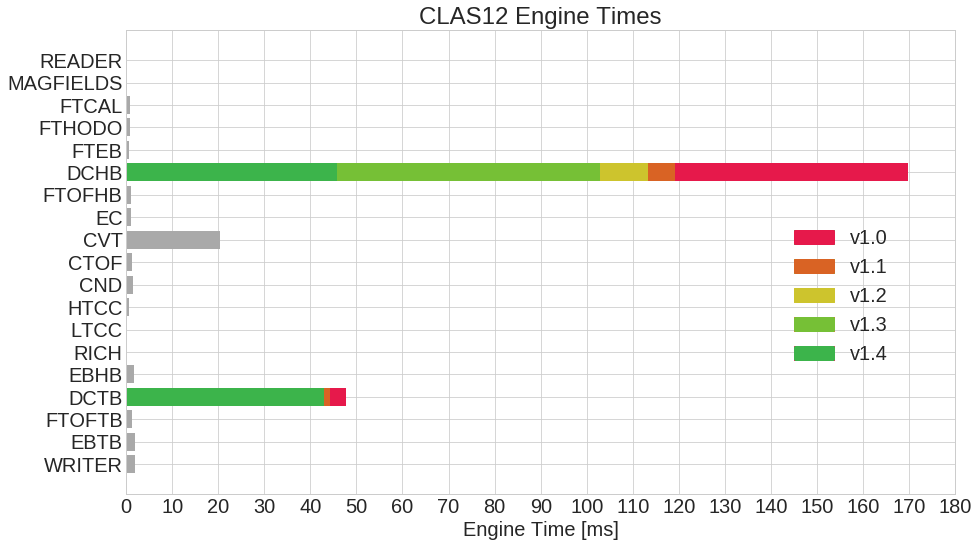
\includegraphics[scale=0.44]{engine_times/1_4}
        \caption{\label{fig:engines_times-final} Engine CPU times.}
    \end{figure}

Regarding the work done for JLab, the improvements on the DCHB and DCTB engines are considerable, as can be seen in Figure \ref{fig:engines_times-final}.
A comprehensive list of each version, it's associated changes to the code, its effect in the total computation time and how useful it is for the community in general follows:
    \begin{itemize}
        \item \textbf{v1.1}: This version consists of the refactoring and optimizations explained in Section \ref{ssec:refactoring_and_optimizations}.
        It's surprising to see that this version brings the largest improvement in computing time, considering that the changes done only apply to the quality of the coding itself and were not changes to the algorithms themselves.

        This odd behaviour is explained by two main reasons: First, the changes reduce a large amount of unnecessary computations.
        Second and more importantly, the fact that the code was simplified allowed the Java HotSpot Performance Engine to apply heavier dynamic optimizations in runtime to the program~\cite{hunt2011java}.
        
        While this version provides a large improvement for the CLAS12 software, its implementation is mostly only useful for JLab since it is a direct quality improvement of their code and doesn't mean any change for the community in general. % Note: Maybe I should be more detailed when talking about ``the community''?
        
        \item \textbf{v1.2}: This version consists on the implementation of different algorithms to improve the way matrices are handled by the Kalman Filter.
        This change doesn't provide a very significative improvement to the total computing time of CLAS12, which is attributed mostly to the matrix library used in the software, JAMA.
        While the changes brought heavily reduce the complexity of the operations completed in the software as is evidenced in Section \ref{ssec:prop_matrices}, they also require a higher amount of matrices to be initialized, which isn't too efficient in the library~\cite{hicklin2000jama}. % Note: I could add a figure that evidences this. If I look at the matrices computations while profiling it can be seen that around 9% of the total time spent is spent initializing matrices.
        
        However, the changes applied could produce a bigger improvement for other particle detectors' software or for other instances of the EKF, considering that the need for matrix inversions and multiplications is completely eliminated in the Update phase of the filter.
        A potential future work that is proposed to reap the benefit of the work done in this version would be to switch to another matrix library or implement a new one that takes better advantage of these changes.
        
        \item \textbf{v1.3}: This version relates to the implementation of a magnetic field interpolation algorithm as is described in Section \ref{ssec:prop_magfield}.
        Again, this change doesn't provide a very big difference on the final computing time of DCHB, but it has the advantage of producing such improvements with minimal effect on the precision of the results.
        As for the benefit that this work could provide for the community in general, its potential is limited by its use; while other publications provide interpolation methods with much higher accuracy~\cite{mackay2006divergence}, this one provides very quickly computed results which can be accurate enough for certain applications, as can be seen in Figure \ref{fig:bfield_slice}.
        
            \begin{figure}[ht]
                \centering
                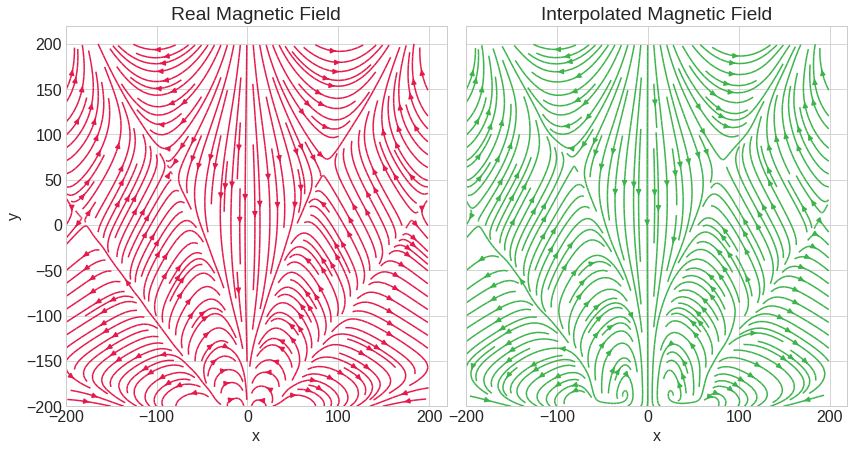
\includegraphics[scale=0.515]{bfield/bfield_slice}
                \caption{\label{fig:bfield_slice} Vertical cut through the magnetic field transverse to the beam line at $z=500$ [cm].}
            \end{figure}

        \item \textbf{v1.4}: This version simply shows an exploitable capability of particle detectors, which is that many hit clustering and particle tracking algorithms that are currently employed for particle detectors work with independent tracks, and thus are easily parallelizable~\cite{blum2008particle}.
        
        \item \textbf{Additional developments}: The work presented in subsection \ref{ssec:prop_multithreaded_kf}, while not implemented in CLAS12 due to specific constraints, provides useful insight into they improvement they could bring to other particle detectors.
        
        \newpage
        
        The alternative of utilizing the multithreaded KF algorithm proposed can potentially find better final tracks found if the additional computing time can be spared.
        Also, if more time is given to fine-tune this algorithm, it has the potential of improving computing time by analyzing different tracks with less KF iterations, thus diversifying the space used for initial state vectors.
    \end{itemize}

% PROPOSED FUTURE WORK
During the development of this project, some ideas were not evaluated or implemented because they fell out of the scope of this work or because they were not useful in the specific case of CLAS12, but may be useful for other particle detectors that employ Drift Chambers.
A list of these is offered with the hope that they will be investigated in future works:

    \begin{itemize}
        \item \textbf{Fourth Order Adams-Bashforth-Moulton method}: As can be seen in Figure \ref{fig:dc_horizontal_cut} from Section \ref{ssec:framework_dc}, the measurements can be divided in three regions due to the geometry of the detector.
        While most of the distances between measurements are usually at most $4$ or $5$ [cm], the distance between regions can be more than a meter.
        Also, due to the way that the Kalman Filter works, after transporting the state vector from the first measurement site to the last, this vector needs to be transported back to run the KF again, which requires it to be moved for around $3.5$ meters, or the entire length from sector $3$ to sector $1$.
    
\newpage

        Currently, this movement of the state vector is done through Runge Kutta 4, as is described in Section \ref{ssec:framework_dc} with a step size $h=1$ so that the $z$ variable is updated by one centimeter in each RK4's iteration, occasionally updating it by $2$ [cm] when the magnetic field at that point is small enough.
        Considering that for most particles the majority of the movement from regions $1$ to $2$, $2$ to $3$ and from $3$ back to $1$ the step size is kept at $1$ [cm], the option of switching RK4 for the Fourth order Adams-Bashforth-Moulton (ABM4) method for these intervals is evaluated.

        ABM4 is a multi-step method used to solve initial value problems described in detail in Appendix \ref{add:abm4}.
        The method can solve the same kind of problems as RK4, but it has the advantage that it only requires to evaluate the $\mathbf{f}(z,\mathbf{x})$ function twice per iteration, whereas RK4 does this four times.

        The change does not come without disadvantage however, since it requires the use of four previous steps to compute the next one as can be seen in equations \eqref{eq:abm4_explicit} and \eqref{eq:abm4_implicit} from the appendix.
        Due to this the step size must be kept constant through each step, and RK4 needs to be ran for three steps after the initial state vector.
        It's worth noting that due to the particular conditions of the problem, $z_{k+1}$ does not necessarily fulfill the condition that $z_{k+1} = z_k + n h$ where $n$ is an arbitrary natural number, so it's usually impossible to reach the next measurement site from the last one using ABM4, but this can be fixed easily by using RK4 between the last step reached by ABM4 and the measurement plane $z_{k+1}$.

        Due to specific difficulties and time constraints this option was programmed but not implemented, but it's considered a valuable option for future work.
    
        \item \textbf{Split cluster filtering}: While working with the software, it was observed that some split clusters separated using the cluster splitting algorithm described in Section \ref{ssec:framework_cf} are actually produced by what looks like one or a few particles and a large amount of noise.
        The split clusters then go through the track finding algorithm described in Section \ref{ssec:framework_tf} normally and a large portion of time is spent fitting each separately to then be scrapped as noise.
        
        This time could potentially be reduced by running a special track finding algorithm that analyzes them with more scrutiny before running the rest of the algorithm.
        Another option would be trying to fine tune the parameters in the cluster splitting algorithm so that, ideally, these noise clusters would be removed before it is attempted to find tracks from them.
    
        \item \textbf{Magnetic field interpolation parameter tuning}: Regarding the magnetic field interpolation proposed in Section \ref{ssec:prop_magfield}, the parameter tuning could use much more work which was not considered due to the large amount of time the tests would take.
        The option of fine tuning each parameter separately opens the possibility of a more precise or faster implementation by offering a smaller step size in some dimensions or different ranges for the $x$ and $y$ variables.
        
        \item \textbf{Alternate magnetic field interpolation methods}: Attention is also brought to the fact that only trilinear interpolation is used.
        Triquadratic or tricubic interpolation might produce more accurate results, but they were not attempted due to the fact that they could potentially be far slower than the original implementation, which would work against the original objective of interpolating the field in the first place.
        
        \item \textbf{Kalman Filter Fine Tuning}: The EKF implemented in CLAS12 works with various parameters, like the number of iterations, the Runge-Kutta 4 original step size and its criteria for increasing this step size, the convergence criteria for stopping the filter before reaching the maximum number of iterations, and the newly introduced number of iterations using the interpolated magnetic field.

        All of these parameters were set somewhat haphazardly, by trial and error.
        The option of running another Kalman Filter that trains the original one by fine-tuning these parameters is proposed, with the alternative of using methods from machine learning, which has already been done in the academy~\cite{abbeel2005discriminative}.
        
        \item \textbf{Hough-Transform-based cluster finding}: An option that was considered but quickly discarded due to time constraints is that of using the Hough Transform (described in Appendix \ref{add:hough_transform}) over the set of all the hits in one event instead of only to split clusters.
        
        While this option would probably be slower in CPU, it offers the possibility of leveraging this computation to a GPU, which has already been proved possible~\cite{braak2011fast}, even for the specific case of particle accelerators, such as the LHC~\cite{halyo2013gpu}.
        
        \item \textbf{FPGA-or-ASIC-based cluster finding}: Another option that was considered but not tried is that of migrating the cluster finding described in Section \ref{ssec:framework_cf} to hardware via Field Programmable Gate Arrays (FPGAs) or Application-Specific Integrated Circuits (ASICs).
        The proposal comes from the fact that the Clump Finding and Hit Pruning parts of the algorithm are very basic and can be done without any floating-point computation, task that famously can be hard for FPGAs~\cite{fagin1994field}.
        
        It might even be possible to run the whole cluster finding algorithm in FPGAs by discovering a good implementation of the \textbf{Cluster Fitting} and \textbf{Cluster Splitting} parts of the algorithm that don't heavily rely on floating-point operations.
    \end{itemize}

Special attention is brought again to the fact that the biggest improvement in the code is seen in version $1.1$, the ``code clean-up''.
The refactoring done was not completely thorough, and perhaps even larger changes can be obtained by reworking the DC software by rewriting most classes from the algorithm up.

\newpage

A final reflection on this same subject relates to the language choice for the CLAS12 software, Java.
In the current programming environment, where processing units' focus is shifting from complex and fast general purpose CPUs to lower-power, multi-core processor units, the software should be adapting alongside the hardware and a shift to languages with small memory footprint and well-defined states should be preferred.
This change of focus can be seen, for example, in the software development for the LHC, where clear guidelines have been stated to switch software to C++~\cite{foundation2017roadmap} and to use simpler date structures, drifting away from the objects common to object-oriented programming~\cite{cerati2016kalman}.

While originally the choice of using Java might have made sense, in the current context of high performance computing this option is disputed.
It has been repeatedly proven that C/C++ provides at least double the computing speed of Java and at most a quarter of the memory usage~\cite{prechelt2000empirical}, with even larger differences found in other studies~\cite{prechelt1999comparing}.
Changing the codebase to C/C++ can even be aided by the computing framework, CLARA, due to the fact that it supports services in both Java and C++~\cite{gyurjyan2013clara}, which means that the change could be applied gradually; thus allowing for incremental tests to be applied while this change is taking place.